% !TeX spellcheck = hu_HU
% !TeX encoding = UTF-8

%----------------------------------------------------------------------------
\appendix
%----------------------------------------------------------------------------
\chapter*{\fuggelek}\addcontentsline{toc}{chapter}{\fuggelek}
\setcounter{chapter}{\appendixnumber}
%\setcounter{equation}{0} % a fofejezet-szamlalo az angol ABC 6. betuje (F) lesz
\numberwithin{equation}{section}
\numberwithin{figure}{section}
\numberwithin{lstlisting}{section}
%\numberwithin{tabular}{section}
%
%%----------------------------------------------------------------------------
\section{Linda típusok}

Az alábbi táblázat tartalmazza a jelenlegi Linda megvalósítás által biztosított Linda típusokat, illetve a hozzájuk tartozó sorosítási megvalósítást.

\begin{table}[h!]
    \begin{tabularx}{\linewidth}{|l|l||c|X|}
        \hline
        \textbf{C++ típusnév} & \textbf{Típus} & \textbf{Kód} & \textbf{Tartalom} \\
        \hline
        \texttt{std::int16\_t} & 16--bites előjeles egész & $0$ & A szám értéke \\\hline
        \texttt{std::uint16\_t} & 16--bites előjel nélküli egész & $1$ & A szám értéke \\\hline
        \texttt{std::int32\_t} & 32--bites előjeles egész & $2$ & A szám értéke \\\hline
        \texttt{std::uint32\_t} & 32--bites előjel nélküli egész & $3$ & A szám értéke \\\hline
        \texttt{std::string} & sztring & $4$ & A sztring bájtjainak száma (64--biten előjel nélkül), majd annak bájtjai \\\hline
        \texttt{ldb::lv::fn\_call} & függvényhívás & $5$ & A függvény neve mint sztring, majd rekurzívan \nes{}ként a paraméterei \\\hline
        \texttt{std::int64\_t} & 64--bites előjeles egész & $6$ & A szám értéke \\\hline
        \texttt{std::uint64\_t} & 64--bites előjel nélküli egész & $7$ & A szám értéke \\\hline
        \texttt{single} & egyszeres lebegőpontos szám & $8$ & A szám értéke \\\hline
        \texttt{double} & kétszeres lebegőpontos szám & $9$ & A szám értéke \\\hline
        \texttt{ldb::lv::type\_ref} & típus referencia & $A$ & A hivatkozott típus kódja 8--biten \\\hline
    \end{tabularx}
    \caption{A típusok sorosítási értékei}
    \label{tbl:type-serial}
\end{table}

\section{Megoldások}

\subsection{Csatorna alapú kommunikáció}\label{x:subsec:sln-csp}

\begin{lstlisting}[label=lst:ex-csp-buf, caption={Példa a Linda alatt megvalósított CSP csatornákra (1)},gobble=2,language=C,numbers=left]
	using channel_t = std::string_view;

	channel_t
	make_channel(std::string_view channel) {
		out(channel);
		return channel;
	}

	void
	enq_msg(channel_t channel, std::string x) { // itt string, de általánosítható
		in(channel);
		out(channel, x);
	}

	int
	deq_msg(channel_t channel) {
		int val;
		in(channel, ldb::ref(&val));
		out(channel);
		return val;
	}

	int
	read_file(channel_t outch, std::string n) {
		std::istream fin(path);
		std::string data;
		while (std::getline(fin, data)) {
			enq_msg(outch, data);
		}
		enq_msg(outch, ""); // empty string marks EOF
		return 0;
	}

	int
	real_main(int argc, char** argv) {
		const auto ch = make_channel("file-data");

		int inputs = argc - 1; // feltéve helyes bemenetet
		for (int i = 1; i < argc; ++i) {
			eval(i, (read_file)(ch, argv[i]));
		}

		std::uint64_t words = 0;
		std::uint64_t lines = 0;
		std::uint64_t chars = 0;
		for (;;) {
			const auto next = deq_msg(ch);
			if (next.empty()) {
				if (inputs == 1) break; // end if all files finished
				--inputs;
				continue;
			}
			words += count_words(next);
			++lines;
			chars += next.size();
		}
		std::cout << words << ' ' << lines << ' ' << chars << '\n';
		for (int i = 1; i < argc; ++i) {
			in(i, 0);
		}
		return 0;
	}
\end{lstlisting}


\begin{lstlisting}[label=lst:ex-csp-unbuf, caption={Példa a Linda alatt megvalósított CSP csatornákra (2)},gobble=2,language=c,numbers=left]
	using channel_t = std::string_view;

	channel_t
	make_channel(std::string_view channel) {
		out("_CNTR", channel, 0U);
		out("_READ", channel, 0U);
		return channel;
	}

	void
	enq_msg(channel_t channel, std::string x) { // itt string, de általánosítható
		unsigned cntr;
		in("_CNTR", channel, ldb::ref(&cntr));
		out(channel, cntr, x);
		out("_CNTR", channel, cntr++);
	}

	std::string
	deq_msg(channel_t channel) {
		unsigned read;
		in("_READ", channel, ldb::ref(&read));
		std::string val;
		in(channel, read++, ldb::ref(&val));
		out("_READ", channel, read);
		return val;
	}

	int
	read_file(channel_t outch, std::string path) { ... }

	int
	real_main(int, char**) { ... }
\end{lstlisting}

\subsection{Szemaforok}\label{x:subsec:sln-semaphore}

\begin{lstlisting}[gobble=2,language=C,numbers=left,caption={Példa szemafor megvalósítás}]
	int
	new_lsemaphore(int with_max = 1) {
		int last = 0;
		inp("__SEM_CNTR", ldb::ref(&last)); // stays 0 if lookup fails (i.e. first call)

		int current = last + 1;
		out("__SEM_CNTR", current);
		out("__SEM_STATE", current, with_max);
		return current;
	}

	void
	acquire_lsemaphore(int sem_handle) {
		int current = 0;
		in("__SEM_STATE", sem_handle, ldb::ref(&current));
		while (current == 0) {
			// clear previously set signal on the semaphore
			inp("__SEM_SIGNAL", sem_handle);
			out("__SEM_STATE", sem_handle, 0);
			in("__SEM_SIGNAL", sem_handle);
			in("__SEM_STATE", sem_handle, ldb::ref(&current));
		}
		out("__SEM_STATE", sem_handle, current - 1);
	}

	void
	release_lsemaphore(int sem_handle) {
		int current = 0;
		in("__SEM_STATE", sem_handle, ldb::ref(&current));
		out("__SEM_STATE", sem_handle, current + 1);
		out("__SEM_SIGNAL", sem_handle);
	}
\end{lstlisting}

%%----------------------------------------------------------------------------
%\begin{figure}[!ht]
%\centering
%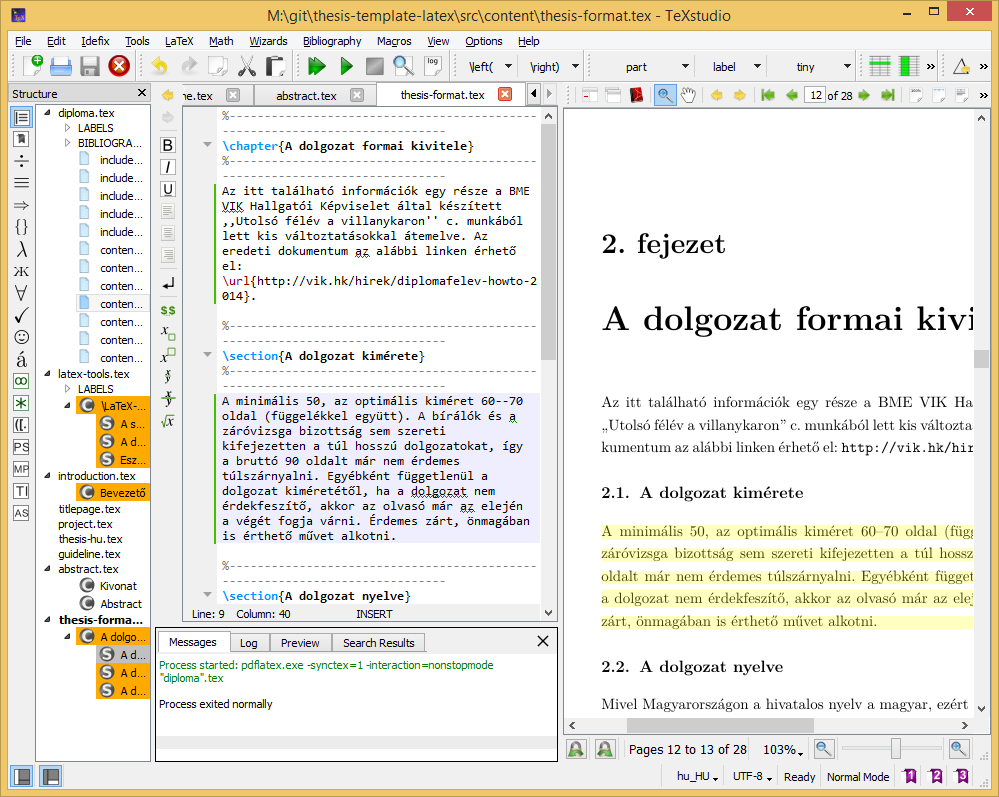
\includegraphics[width=150mm, keepaspectratio]{figures/TeXstudio.png}
%\caption{A TeXstudio \LaTeX-szerkesztő.}
%\end{figure}
%
%%----------------------------------------------------------------------------
%\clearpage\section{Válasz az ,,Élet, a világmindenség, meg minden'' kérdésére}
%%----------------------------------------------------------------------------
%A Pitagorasz-tételből levezetve
%\begin{align}
%c^2=a^2+b^2=42.
%\end{align}
%A Faraday-indukciós törvényből levezetve
%\begin{align}
%\rot E=-\frac{dB}{dt}\hspace{1cm}\longrightarrow \hspace{1cm}
%U_i=\oint\limits_\mathbf{L}{\mathbf{E}\mathbf{dl}}=-\frac{d}{dt}\int\limits_A{\mathbf{B}\mathbf{da}}=42.
%\end{align}
